% !TeX root = ../../../main.tex
\begin{figure}[!htbp]
\ChThreeFloatContents
  {ch03:fig:first_event_time}
  {\caption{ (a)-(b) Distribution of Time of First Composite Adverse Event (in Months) across Patients Stacked by Each Adverse Event Type. 
  (a) includes patients with no adverse event (Right-Censored). 
  (b) presents the histogram of times only for patients with an adverse event recorded (Excluding Right-Censored Patients).
  (c)-(d) Distribution of Event Types within each Composite Adverse Event.}}
  {%
    \subfigure[All Patients]{\label{ch03:fig:first_event_time_with_censoring}%
      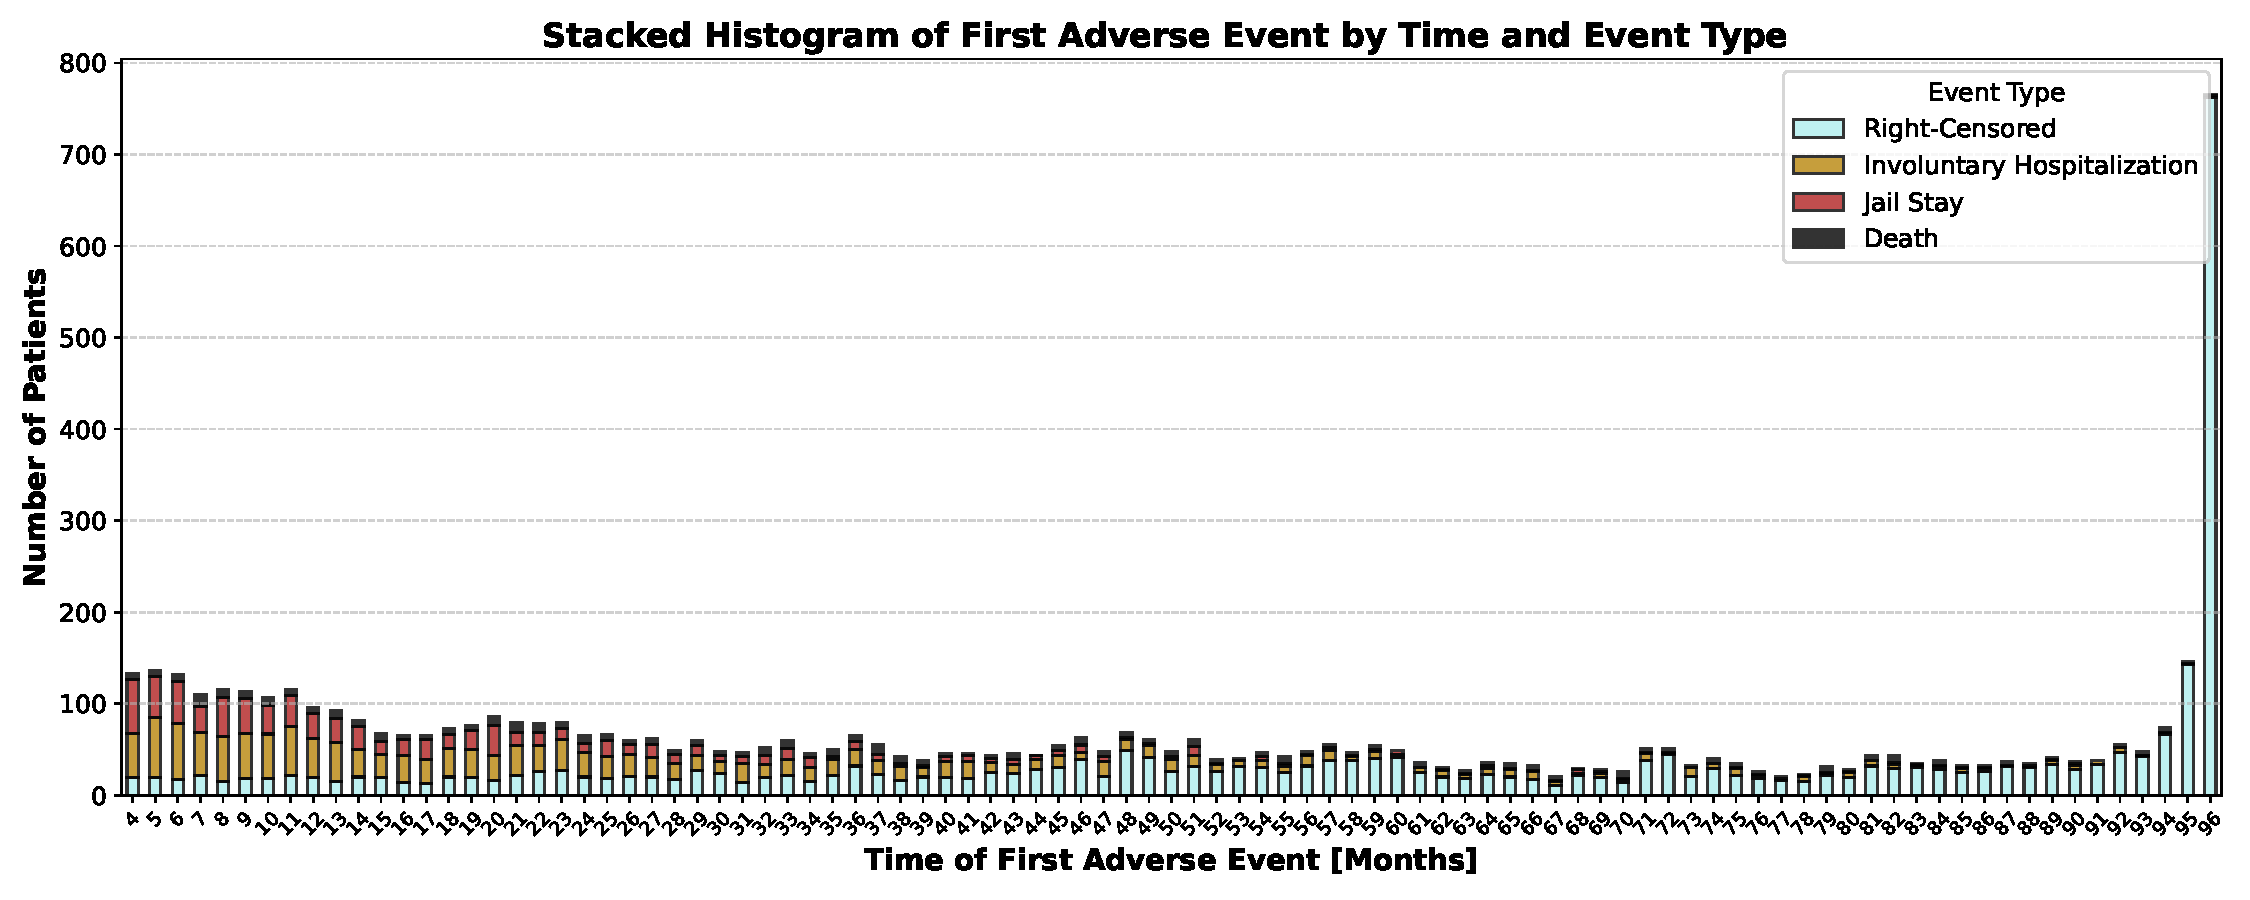
\includegraphics[width=0.9\linewidth]{Appendices/appendix-ch03/images/First_Event/first_event_time_histogram.pdf}}%
    \\
    \subfigure[Patients with an Adverse Event]{\label{ch03:fig:first_event_time_without_censored_data}%
      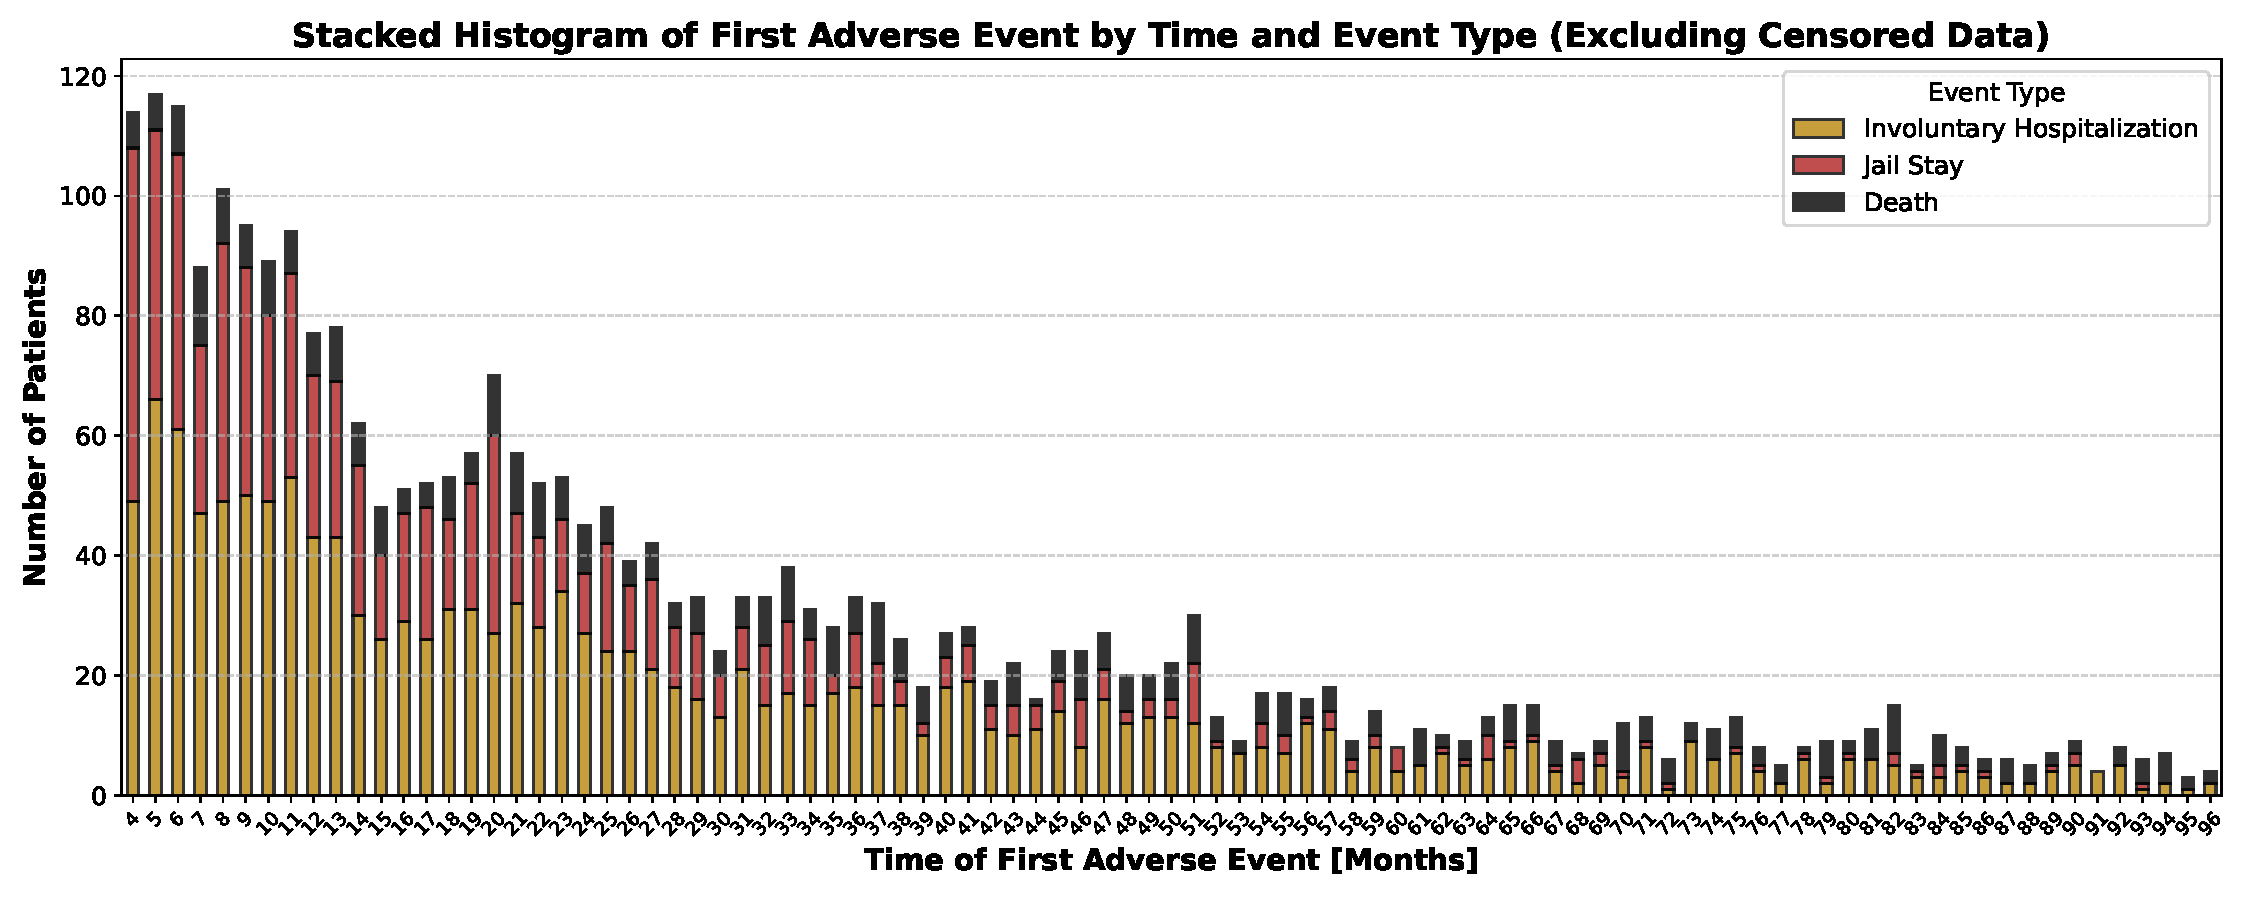
\includegraphics[width=0.9\linewidth]{Appendices/appendix-ch03/images/First_Event/first_event_time_histogram_exclude_no_event.pdf}}%
    \\
    \subfigure[Event Type Distribution - All Patients]{\label{ch03:fig:event_type_with_censoring}%
      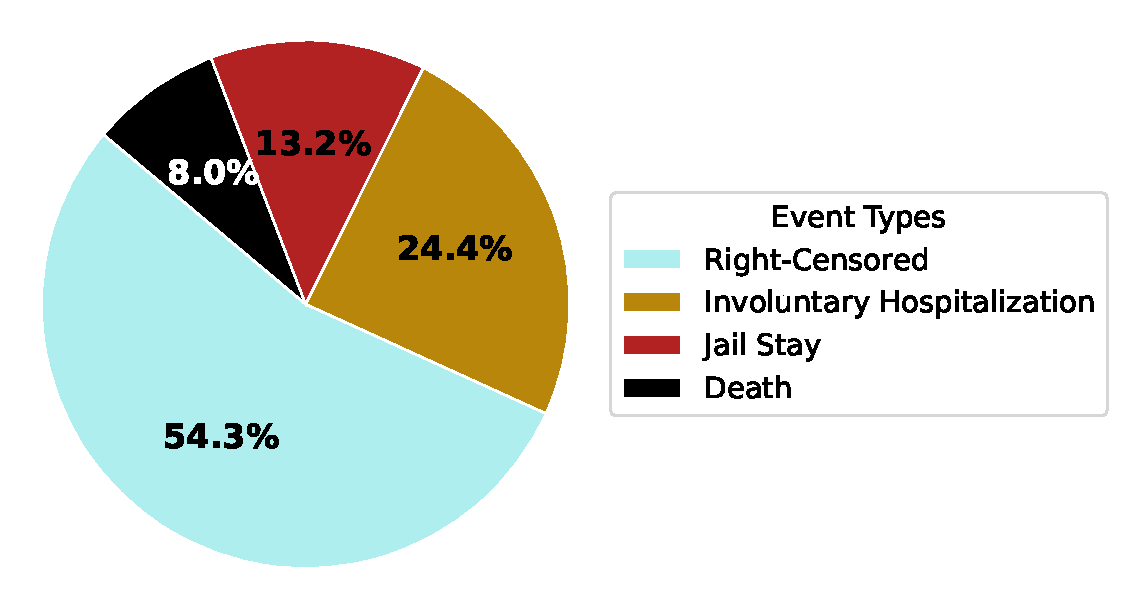
\includegraphics[width=0.4\linewidth]{Appendices/appendix-ch03/images/First_Event/first_event_type_piechart.pdf}}%
    \qquad
    \subfigure[Event Type Distribution - Patients with an Adverse Event]{\label{ch03:fig:event_type_without_censored_data}%
      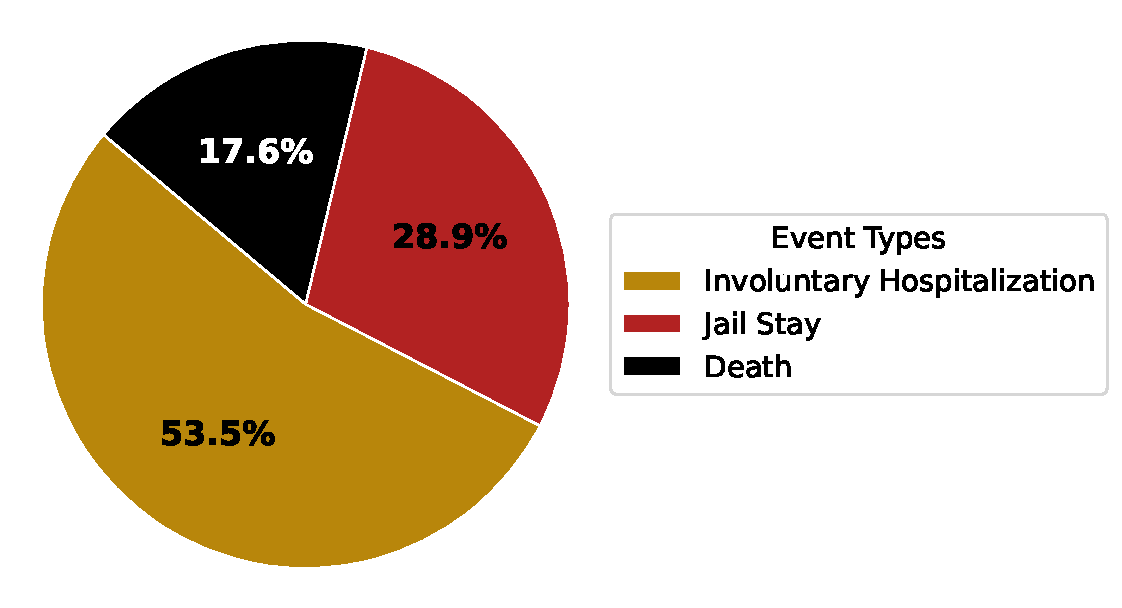
\includegraphics[width=0.4\linewidth]{Appendices/appendix-ch03/images/First_Event/first_event_type_piechart_exclude_no_event.pdf}}%
  }
\end{figure}